%%%%%%%%%%%%%%%%%%%%%%%%%%%%%%%%%%%%%%%%%%%%%%%%%%%%%%%%%%%%%%%%%%%%%%%%%%%%%%
\section{System configuration}

The proposed DAQ system supports multiple run configurations,
as shown in Figure~\ref{figure:run_configurations}.

\begin{figure}[H]
  \begin{tikzpicture}
    \node[anchor=south west,inner sep=0] at (0,0.) {
      % \node[shift={(0 cm,0.cm)},inner sep=0,rotate={90}] at (0,0) {}
      \makebox[\textwidth][c] {
        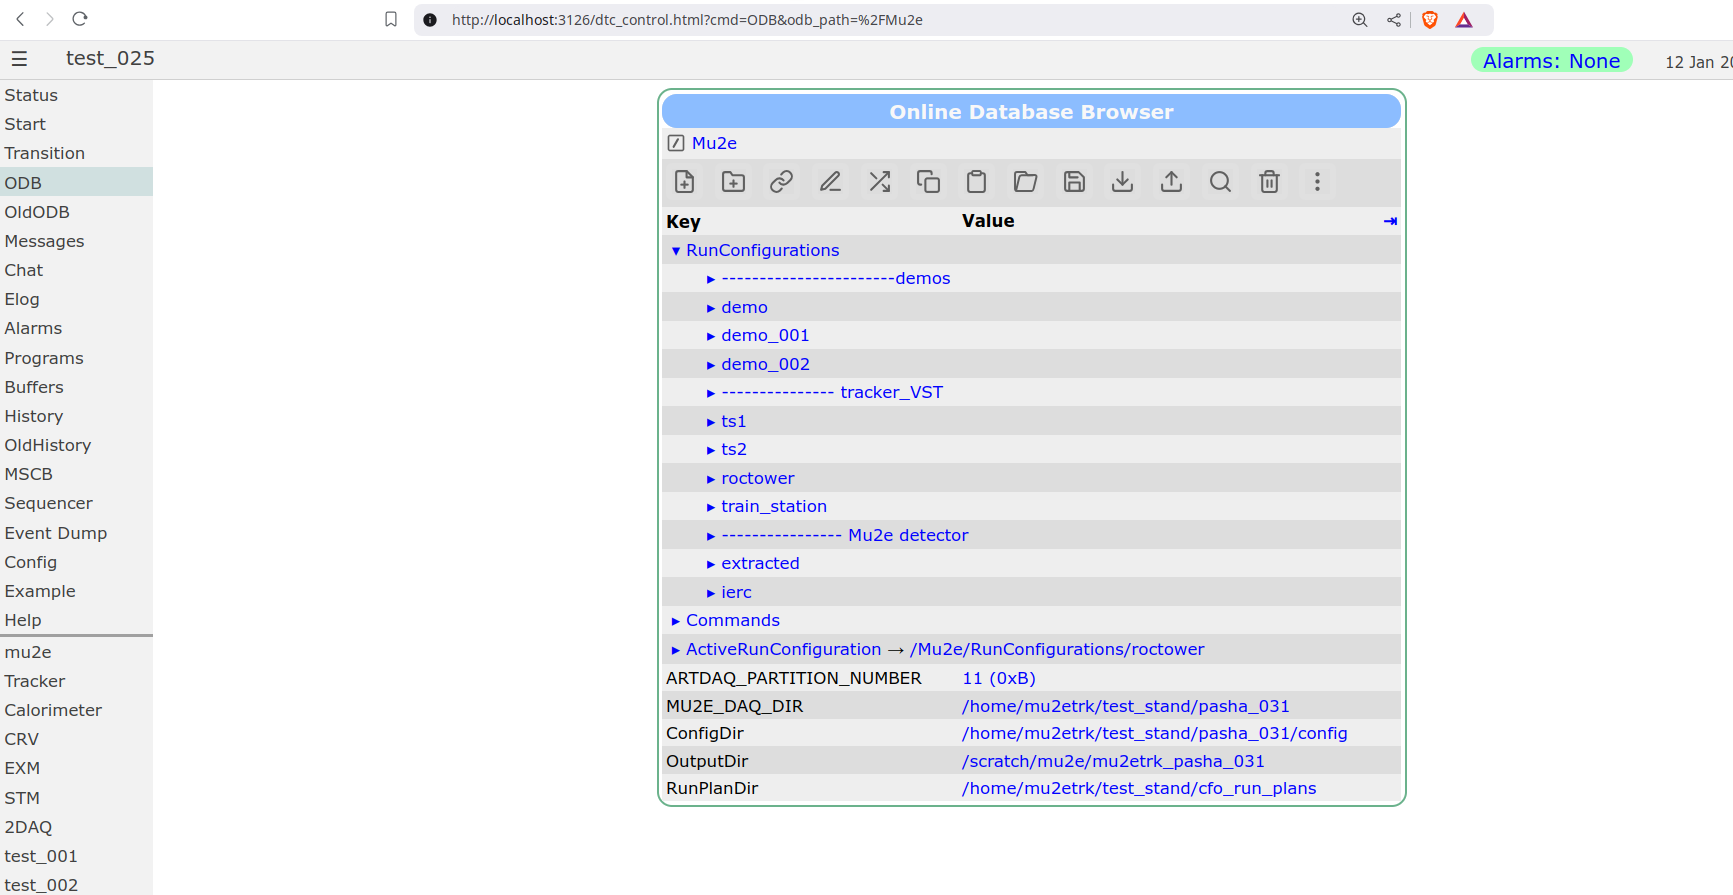
\includegraphics[width=0.95\textwidth]{png/run_configurations}
      }
    };
    % \node [text width=8cm, scale=1.0] at (14.5,0.5) {$\mu_B$, expected background mean};
    % \node [text width=8cm, scale=1.0, rotate={90}] at (1.5,7.5) { $S_{D}$, ``discovery'' signal strength  };
  \end{tikzpicture}
  \caption{
    \label{figure:run_configurations}
    Top-level run configurations
  }
\end{figure}

\begin{itemize}
\item 
  Run configurations are stored in the "/Mu2e/RunConfigurations" ODB subtree
\item
  each run configuration is an independent subtree, so any modification
  of a given run configuration doesn't affect other run configurations
\item
  a run configuration template can be saved as a .json structure and loaded from
  an external .json file, for example
\begin{verbatim}
mu2etrk@mu2edaq22:~/test_stand/pasha_031>odbedit
[local:test_025:S]/>cd Mu2e/Run
[local:test_025:S]/>cd Mu2e/RunConfigurations/demo
[local:test_025:S]demo>save demo.json
[local:test_025:S]demo>exit
\end{verbatim}
\item
  ODB links are allowed, but have to point within the configuration
\item
  configuration templates are archived on github. 
\end{itemize}

%%%%%%%%%%%%%%%%%%%%%%%%%%%%%%%%%%%%%%%%%%%%%%%%%%%%%%%%%%%%%%%%%%%%%%%%%%%%%%
\subsection{Structure of  the run configuration}
\begin{itemize}
\item 
  a run configuration has a name, a status, a list of elements - subsytem configurations,
  \new{and some global parameters,} as shown in Figure~\ref{figure:configuration_top}
\item
  each subsystem has a separate configuration subtree
\item
  \new{subsystem configuration templates are archived} in the 
  \href{https://github.com/pavel1murat/frontends/tree/main/odb/Mu2e/Subdetectors}
  {\blue frontends/odb/Mu2e/Subdetectors} subdirectory
\item
  Shown in  Figure~\ref{figure:run_configurations} ODB element "/Mu2e/ActiveRunConfiguration" is an ODB link
  pointing to the currently active configuration ("roctower").
\end{itemize}

\begin{figure}[H]
  \begin{tikzpicture}
    \node[anchor=south west,inner sep=0] at (0,0.) {
      % \node[shift={(0 cm,0.cm)},inner sep=0,rotate={90}] at (0,0) {}
      \makebox[\textwidth][c] {
        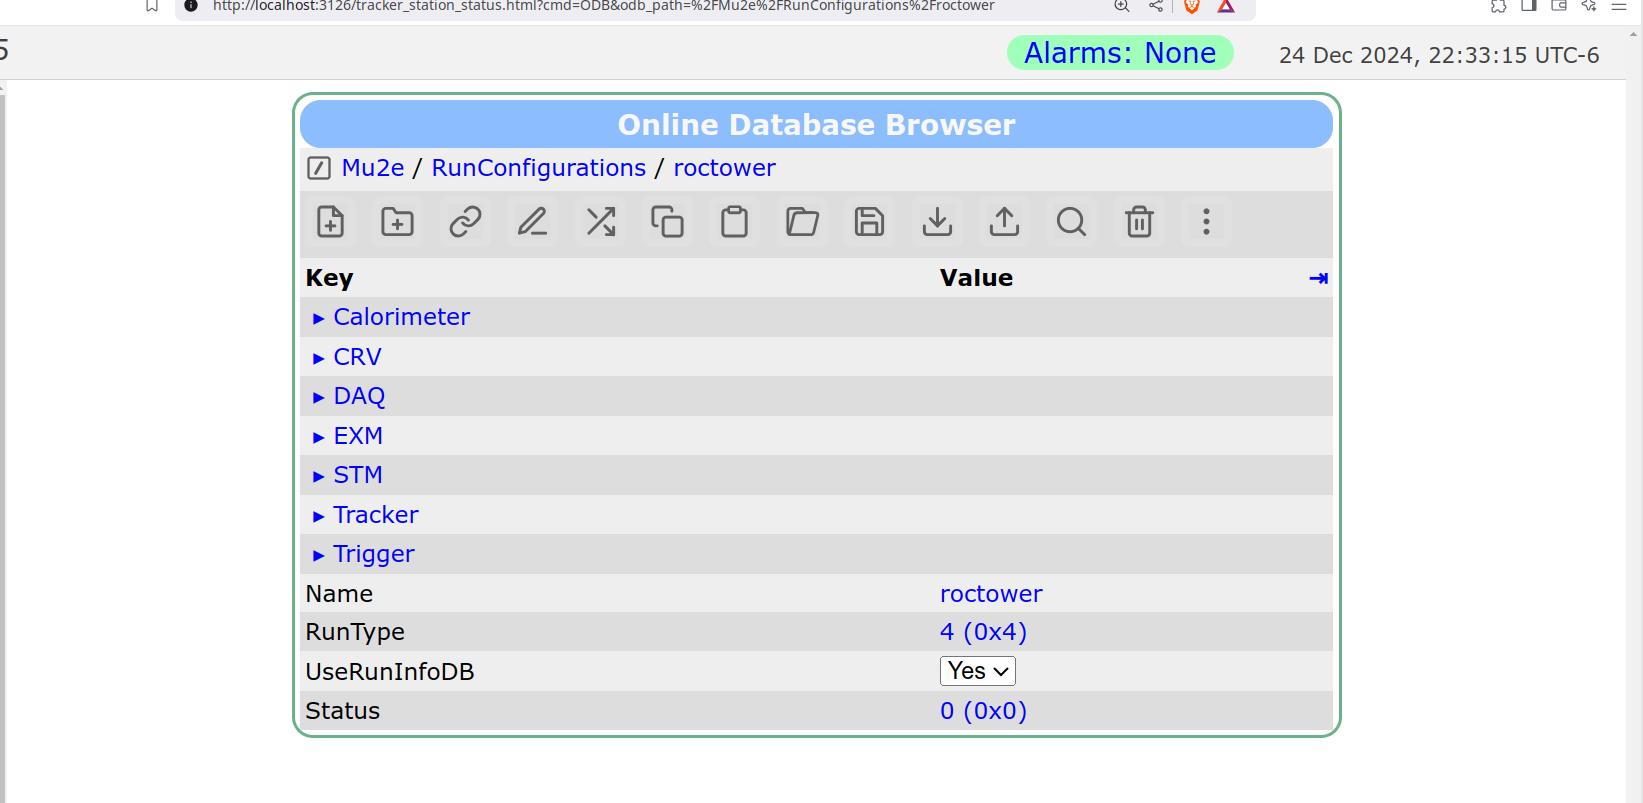
\includegraphics[width=0.95\textwidth]{png/configuration_top}
      }
    };
    % \node [text width=8cm, scale=1.0] at (14.5,0.5) {$\mu_B$, expected background mean};
    % \node [text width=8cm, scale=1.0, rotate={90}] at (1.5,7.5) { $S_{D}$, ``discovery'' signal strength  };
  \end{tikzpicture}
  \caption{
    \label{figure:configuration_top}
    Top view of the configuration called 'roctower' - a 6-ROC tracker test stand in IERC
  }
\end{figure}

%%%%%%%%%%%%%%%%%%%%%%%%%%%%%%%%%%%%%%%%%%%%%%%%%%%%%%%%%%%%%%%%%%%%%%%%%%%%%% 
\subsection{Subsystem configuration}

Each Mu2e subsystem, subdetectors and the DAQ, is represented by its
configuration [sub]tree in the detector configuration.
The configuration trees are subsystem-specific, consist of different elements,
and have different levels of hierarchy.
However, each configuration element has two mandatory parameters, {\bf Enabled}
and {\bf Status}, used for monitoring and error reporting.
Their meaning is as follows 

\begin{itemize}
\item
  {\bf Enabled} = 0: the element (sub-tree) is considered present, but not used.
\item
  {\bf Enabled} = 1: the element is included into the configuration and expected
  to be used
  \begin{itemize}
  \item
    status = 0 : the subsystem is OK
  \item
    status < 0 : the subsystem has a problem and an action is required
    The value of the status variable is the error code
  \item
    status > 0 : the subsystem has a warning-level problem, no immediate action
    is required
  \end{itemize}
\end{itemize}

The following sections describe configurations of the individual subsystems

%%% Local Variables:
%%% mode: latex
%%% TeX-master: t
%%% End:
